\documentclass[a4paper]{article}
\usepackage[T2A]{fontenc}
\usepackage[utf8]{inputenc}
\usepackage[ukrainian]{babel}
\usepackage{tikz}
\usepackage{lastpage} 
\usepackage[left=2.5cm, right=1.5cm, top=1.5cm, bottom=2.5cm]{geometry}
\usepackage{fancyhdr}
% \usepackage{graphicx}

\pagestyle{fancy}
\fancyhf{}
\renewcommand{\headrulewidth}{0pt}
\renewcommand{\footrulewidth}{0pt}
% \pagestyle{empty}

\newcommand{\makrosTitle}[2]{
\thispagestyle{empty}
        \centering
        \textbf{Міністерство освіти і науки України}\\
        \textbf{КИЇВСЬКИЙ ПОЛІТЕХНІЧНИЙ УНІВЕРССИТЕТ}\\[2cm]
        \raggedleft
        Кафедра автоматизації та систем неруйнівного контролю\\
        Група ПМ-11
        \vfill
        \centering
        \textbf{ПРОЕКТУВАННЯ СИСТЕМ АВТОМАТИЗАЦІЇ}\\[1cm]
        \textbf{ЗВІТ З ЛАБОРАТОРНОЇ РОБОТИ №#1}\\[1cm]
        \textbf{#2}
        \vfill
        \begin{flushleft}
            Керівник  \qquad\qquad\quad \hfill\qquad (підпис)\hfill 
            д.т.н., проф. Черепанська І. Ю.\\
            \hfill (дата)\\[2cm]
            Виконавець\hfill (підпис)\hfill Погорєлов Б. Ю.\\
            \hfill (дата)
        \end{flushleft}
        \vfill
        \centering
        2025
}

\newcommand{\makrosFrameBig}[2]{
    \thispagestyle{empty} % Вимикає номер сторінки на першій сторінці
    
    \begin{tikzpicture}[remember picture, overlay]
        \begin{scope}[shift={([xshift = 20 mm, yshift = 10 mm]current page.south west)}]
            \draw[line width=2] (0,0) rectangle (180 mm,277 mm);
        \end{scope}
    \end{tikzpicture}
    
    \begin{tikzpicture}[remember picture, overlay]
        \begin{scope}[shift={([xshift = 20 mm, yshift = 10 mm]current page.south west)}, x=1mm, y=1mm]
            \draw[line width=2] (0,0) rectangle (180,40);
            \draw[line width=2]  (7,40) -- (7, 25);
            \draw[line width=2] (17,40) -- (17, 0);
            \draw[line width=2] (40,40) -- (40, 0);
            \draw[line width=2] (55,40) -- (55, 0);
            \draw[line width=2] (65,40) -- (65, 0);
            \draw[line width=2] (135,25) -- (135,0);
            \draw[line width=2] (140,15) -- (140,20);
            \draw[line width=2] (145,15) -- (145,20);
            \draw[line width=2] (150,25) -- (150,15);
            \draw[line width=2] (165,25) -- (165,15);
        
            \draw (0,35) -- (65, 35);
            \draw[line width=2] (0,30) -- (65, 30);
            \draw[line width=2] (0,25) -- (180, 25);
            \draw (0,20) -- (65, 20);
            \draw (0,15) -- (65, 15);
            \draw (0,10) -- (65, 10);
            \draw (0,5) -- (65, 5);
        
            \draw[line width=2] (135,20) -- (180, 20);
            \draw[line width=2] (135,15) -- (180, 15);
            
            \node at (3.5, 27.5) {Зм.};
            \node at (12, 27.5) {Лист};
            \node at (28.5, 27.5) {№ докум.};
            \node at (47.5, 27.5) {Підпис};
            \node at (60, 27.5) {Дата};
            
            \node at (7, 22.5) {Розроб.};
            \node at (6.5, 17.5) {Перев.};
            \node at (8.5, 7.5) {Н. Контр.};
            \node[align=left] at (5, 2.5) {Затв.};
            
            \node at (142.5, 22.5) {Літ.};
            \node at (157.5, 22.5) {Аркуш};
            \node at (172, 22.5) {Аркушів};
        
            \node[align=left, font=\itshape, anchor=south west, scale=0.9] at (16, 20) {Погорєлов Б.Ю.};
            \node[align=left, font=\itshape, anchor=south west, scale=0.8] at (16, 15) {Черепанська І.Ю.};
            \node[align=left, font=\itshape, anchor=south west, scale=0.8] at (16, 0) {Черепанська І.Ю.};
        
            \node[anchor=center, font=\itshape, scale=1.5] at (122, 32) {#1};
            \node[align=center, font=\itshape, anchor=center] at (100, 12) {#2};
            \node[align=left, font=\itshape, anchor=south west, scale=0.9] at (135, 5) {КПІ ім. І. Сікорського, ПБФ};
            \node[anchor=center, font=\itshape] at (158, 17) {2};
            \node[anchor=center, font=\itshape] at (172, 17) {\pageref{LastPage}};    
        \end{scope} 
    \end{tikzpicture}
}

\newcommand{\makrosFrameSmall}[1]{
    % \thispagestyle{empty} % Вимикає номер сторінки на першій сторінці
    
    \begin{tikzpicture}[remember picture, overlay]
        \begin{scope}[shift={([xshift = 20 mm, yshift = 10 mm]current page.south west)}]
            \draw[line width=2] (0,0) rectangle (180 mm,277 mm);
        \end{scope}
    \end{tikzpicture}
    
    \begin{tikzpicture}[remember picture, overlay]
        \begin{scope}[shift={([xshift = 20 mm, yshift = 10 mm]current page.south west)}, x=1mm, y=1mm]
            \draw[line width=2] (0,0) rectangle (180,15);
            \draw[line width=2] (7,0) -- (7, 15);
            \draw[line width=2] (17,0) rectangle (43,15);
            \draw[line width=2] (55,0) rectangle (64,15);
            \draw[line width=2] (170,0) -- (170, 15);

            \draw[line width=2] (0,5) -- (64, 5);
            \draw               (0,10) -- (64, 10);
            \draw[line width=2] (170,8) -- (180, 8);

            \node[anchor=center, scale=0.8] at (3.5, 2.5) {Змн.};
            \node[anchor=center, scale=0.9] at (12, 2.5) {Арк.};
            \node[anchor=center] at (30, 2.5) {№~докум.};
            \node[anchor=center, scale=0.9] at (49, 2.5) {Підпис};
            \node[anchor=center, scale=0.9] at (59, 2.5) {Дата};
            \node[anchor=center, font=\itshape, scale=1.5] at (115, 7.5) 
                {#1};
            \node[anchor=center] at (175, 12) {Арк.};
            \node[anchor=center] at (175, 4) {\thepage};
            
        \end{scope}
    \end{tikzpicture}
}

% \makrosLab{1}{Шифр}{Назва}
\newcommand{\makrosLab}[3]{ 
    \fancyfoot[C]{\makrosFrameSmall{#2}}
    \makrosTitle{#1}{#3}
    \newpage
    \makrosFrameBig{#2}{#3}
    \raggedright
}


\begin{document}
    \makrosLab{2}{л}{
        Розробка та складання схем \\
        електричних принципових керування \\ 
        промисловими двигунами
    }

    \section*{Тема роботи}
    Розробка та складання схем електричних принципових керування
    промисловими двигунами

    \section*{Мета роботи}
    Вивчити будову та принцип дії промислових двигунів
    різних типів, як складових систем автоматичного
    керування / регулювання / контролю. Навчитися складати схеми електричні
    принципові для керування промисловими двигунами різних типів.

    \section*{Вихідні дані (Варіант 09)}
    \begin{table}[h!]
        \centering
        \begin{tabular}{|l|c|}
            \hline
            \textbf{Параметр} & \textbf{Значення} \\
            \hline
            Потужність, кВт & 1,0 \\
            \hline
            cos$\varphi$ & 0,86 \\
            \hline
            Швидкість обертання n ном, об/хв & 2850 \\
            \hline
            $\gamma$ (перенавантажувальна здатність) & 2,2 \\
            \hline
            ККД, \% & 91 \\
            \hline
            $\alpha$ (кратність пускового струму) & 5,1 \\
            \hline
            $\beta$ (кратність пускового моменту) & 2,35 \\
            \hline
        \end{tabular}
        \caption{Вихідні дані для розрахунків}
    \end{table}

    \newpage 
    
    \section*{Завдання}
Трифазний асинхронний двигун з короткозамкненим ротором має такі параметри:
\begin{enumerate}
    \item напруга живлення: $380/220$ В;
    \item номінальна потужність на валу: $P_{\text{ном.мех}}$;
    \item номінальна швидкість: $n_{\text{ном}}$;
    \item коефіцієнт корисної дії: $\eta$;
    \item коефіцієнт потужності: $\cos \varphi_{\text{ном}}$;
    \item коефіцієнт кратності пускового струму: $\alpha$;
    \item коефіцієнт кратності пускового моменту: $\beta = \frac{M_{\text{пуск}}}{M_{\text{н}}}$;
    \item коефіцієнт перенавантажної здатності: $\gamma = \frac{M_{\text{max}}}{M_{\text{н}}}$.
\end{enumerate}

Двигун увімкнено за схемою "зірка" до мережі з лінійною напругою $U_{\text{лін}} = 380$ В, частотою $f = 50$ Гц.

З врахуванням даних таблиці визначити:
\begin{enumerate}
    \item споживану потужність: активну, реактивну, повну;
    \item споживаний струм;
    \item пусковий струм;
    \item ємність конденсаторів для підвищення $\cos\varphi$ до $0,95$ при вмиканні їх за схемами "зірка" та "трикутник", побудувати векторні діаграми напруги і струмів та трикутник потужностей;
    \item обертаючі моменти двигуна: номінальний, пусковий, критичний;
    \item номінальне і критичне значення ковзання;
    \item обертаючий момент двигуна при значеннях ковзання: $S = 0$; $S_{\text{ном}}$; $0,8S_{\text{кр}}$; $S_{\text{кр}}$; $1,2S_{\text{кр}}$; $0,2$; $0,4$; $0,6$; $0,8$; $1$.
\end{enumerate}
    
    \newpage 
    \section*{Схеми}

\begin{figure}[h]
    \centering
    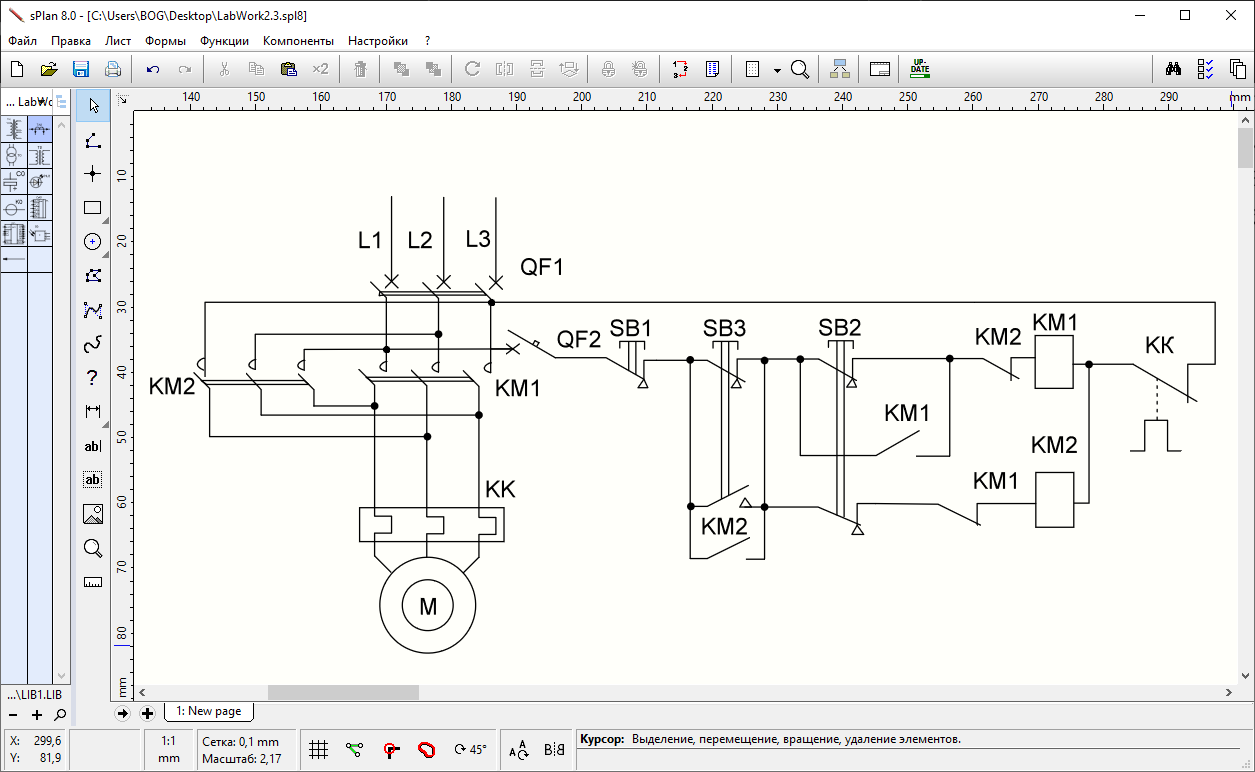
\includegraphics[width=0.45\textwidth]{imgs/LW2.1.png}
    \caption*{Рис. 2.1: Схема електрична принципова реверсивного керування асинхронним електродвигуном}
\end{figure} 

\begin{figure}[h]
    \centering
    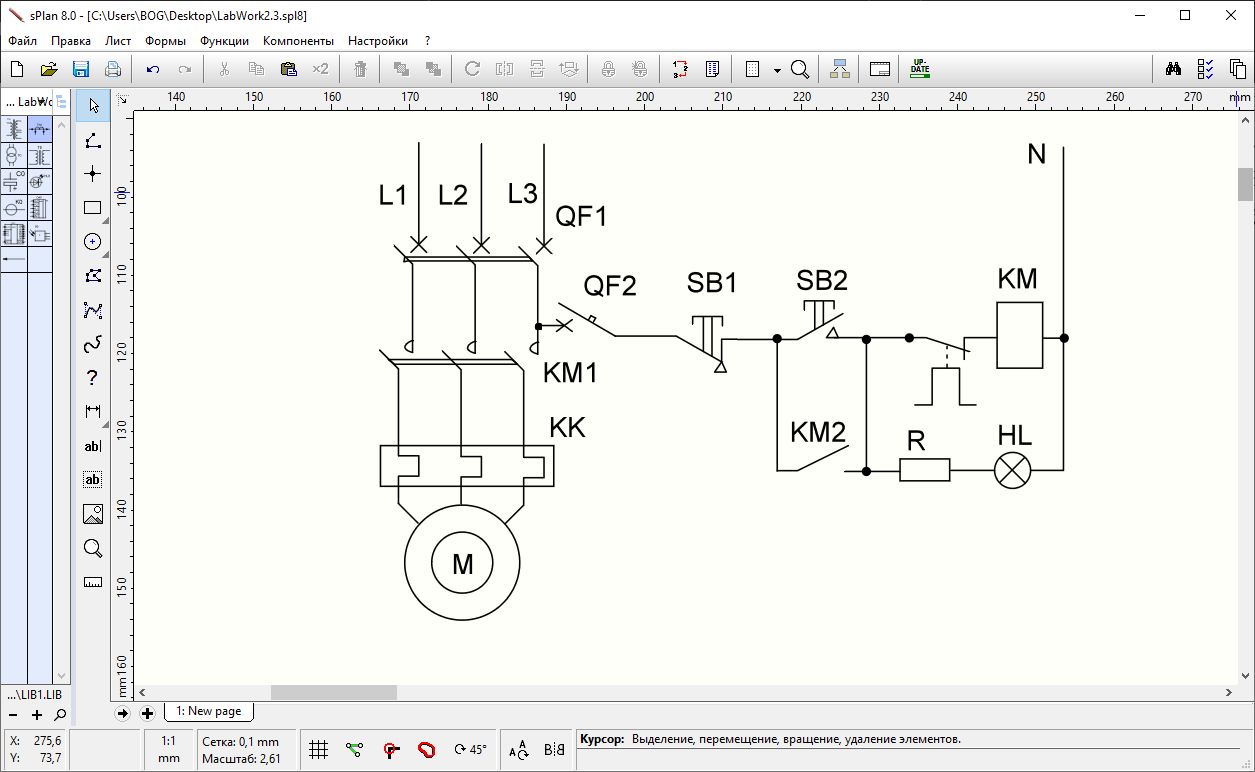
\includegraphics[width=0.5\textwidth]{imgs/LW2.2.png}
    \caption*{Рис. 2.2:Схема електрична принципова нереверсивного керування асинхронним електродвигуном}
\end{figure} 

\begin{figure}[h]
    \centering
    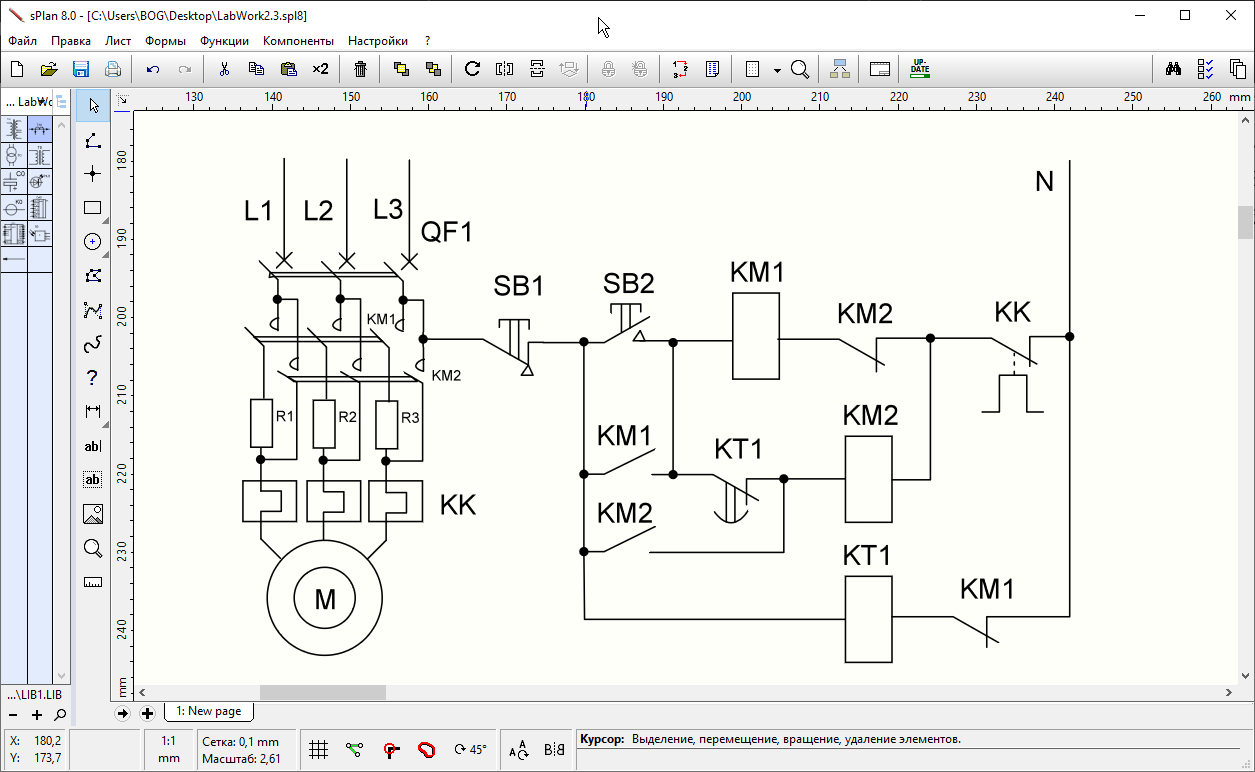
\includegraphics[width=0.5\textwidth]{imgs/LW2.3.png}
    \caption*{Рис. 2.3: Схема електрична принципова керування трифазним асинхронним електродвигуном з короткозамкненим ротором з обмеженням  пускового струму і моменту активними опорами}
\end{figure} 

    \section*{Розрахунки}

\subsection*{Споживана потужність}
\begin{align*}
    P_{\text{спож}} &= \frac{P_{\text{ном.мех}}}{\eta} = \frac{1,0 \text{ кВт}}{0,91} = 1,098 \text{ кВт}.
\end{align*}

\begin{align*}
    S &= \frac{P_{\text{спож}}}{\cos\varphi} = \frac{1,098}{0,86} = 1,277 \text{ кВА}.
\end{align*}

\begin{align*}
    Q &= \sqrt{S^2 - P_{\text{спож}}^2} = \sqrt{1,277^2 - 1,098^2} = 0,635 \text{ кВАр}.
\end{align*}

\subsection*{Споживаний струм}

\begin{align*}
    I &= \frac{S}{\sqrt{3} U_{\text{лін}}} = \frac{1,277 \times 10^3}{\sqrt{3} \times 380} = 1,942 \text{ А}.
\end{align*}

\subsection*{Пусковий струм}

\begin{align*}
    I_{\text{пуск}} &= \alpha I = 5,1 \times 1,942 = 9,9 \text{ А}.
\end{align*}

\subsection*{Обертаючі моменти}

\begin{align*}
    M_{\text{н}} &= \frac{P_{\text{ном.мех}} \times 9550}{n_{\text{ном}}} = \frac{1,0 \times 9550}{2850} = 3,35 \text{ Нм}.
\end{align*}

\begin{align*}
    M_{\text{пуск}} &= \beta M_{\text{н}} = 2,35 \times 3,35 = 7,87 \text{ Нм}.
\end{align*}

\begin{align*}
    M_{\text{кр}} &= \gamma M_{\text{н}} = 2,2 \times 3,35 = 7,37 \text{ Нм}.
\end{align*}

\subsection*{Ковзання}

\begin{align*}
    S_{\text{ном}} &= \frac{n_{\text{с}} - n_{\text{ном}}}{n_{\text{с}}} \approx \frac{3000 - 2850}{3000} = 0,05.
\end{align*}

\begin{align*}
    S_{\text{кр}} &= \frac{M_{\text{н}}}{M_{\text{кр}}} = \frac{3,35}{7,37} = 0,455.
\end{align*}

\subsection*{Ємність конденсаторів}

\begin{align*}
    Q_{\text{кор}} &= P_{\text{спож}} (\tan \varphi_{\text{поч}} - \tan \varphi_{\text{кінц}}) = 1,098 (\tan 30^\circ - \tan 18^\circ) \approx 0,256 \text{ кВАр}.
\end{align*}

\begin{align*}
    C &= \frac{Q_{\text{кор}}}{2 \pi f U^2} = \frac{0,256 \times 10^3}{2 \pi \times 50 \times (380)^2} = 5,7 \text{ мкФ}.
\end{align*}

\section*{Висновки}

Отримані результати дозволяють оцінити параметри роботи трифазного асинхронного двигуна, його енергетичні характеристики та вибір необхідних ємностей для підвищення коефіцієнта потужності.

\section*{Контрольні питання}
\begin{enumerate}
    \item Чому асинхронний двигун так називається? \\
    Асинхронний двигун називається так тому, що частота обертання його ротора не співпадає з частотою обертання магнітного поля статора (яка визначається частотою змінного струму). Різниця між цими частотами називається ковзанням.
    
    \item Чому є небажаною велика сила пускового струму? \\
    Велика сила пускового струму небажана, оскільки вона може призвести до значних механічних та електричних навантажень на двигун і мережу, викликати пошкодження ізоляції проводів, зменшити термін служби обладнання, а також викликати перевантаження трансформаторів і підстанцій.
    
    \item Що використовують для зниження сили пускового струму? \\
    Для зниження сили пускового струму використовують спеціальні пристрої, такі як стартери з обмеженням струму, трансформатори з регульованим напругою або пристрої плавного пуску, що забезпечують поступове збільшення напруги на двигуні.
\end{enumerate}


\end{document}